%%%%%%%%%%%%%%%%%%%%%%%%%%%%%%%%%%%%%%%%%%%%%%%%%%%%%%%%%%%%%%%%%%
%%%%%%%% ICML 2015 EXAMPLE LATEX SUBMISSION FILE %%%%%%%%%%%%%%%%%
%%%%%%%%%%%%%%%%%%%%%%%%%%%%%%%%%%%%%%%%%%%%%%%%%%%%%%%%%%%%%%%%%%

% Use the following line _only_ if you're still using LaTeX 2.09.
%\documentstyle[icml2015,epsf,natbib]{article}
% If you rely on Latex2e packages, like most moden people use this:
\documentclass{article}

% use Times
\usepackage{times}
% For figures
\usepackage{graphicx} % more modern
%\usepackage{epsfig} % less modern
\usepackage{subfigure} 
\usepackage{amsmath,amsfonts,amssymb,bbm}
\usepackage{tikz}
\usetikzlibrary{fit,positioning}

% For citations
\usepackage{natbib}

% For algorithms
\usepackage{algorithm}
\usepackage{algorithmic}

% As of 2011, we use the hyperref package to produce hyperlinks in the
% resulting PDF.  If this breaks your system, please commend out the
% following usepackage line and replace \usepackage{icml2015} with
% \usepackage[nohyperref]{icml2015} above.
\usepackage{hyperref}

% Packages hyperref and algorithmic misbehave sometimes.  We can fix
% this with the following command.
\newcommand{\theHalgorithm}{\arabic{algorithm}}
\DeclareMathOperator{\Tr}{Tr}
\newcommand{\R}{\mathbbm{R}}
\newcommand{\mba}{\mathbf{a}}
\newcommand{\mbb}{\mathbf{b}}
\newcommand{\mbx}{\mathbf{x}}
\newcommand{\mbxt}{\tilde{\mathbf{x}}}
\newcommand{\Sigmat}{\tilde{\Sigma}}
\newcommand{\mbz}{\mathbf{z}}
\newcommand{\mbw}{\mathbf{w}}
\newcommand{\mcN}{\mathcal{N}}
\newcommand{\mcP}{\mathcal{P}}
\newcommand{\mcX}{\mathcal{X}}
\newcommand{\eps}{\epsilon}
\newcommand{\trans}{\intercal}
\newcommand{\Ut}{\tilde{U}}
\DeclareMathOperator*{\argmax}{arg\,max}
\newcommand{\angstrom}{\textup{\AA}}
\newcommand{\red}[1]{\textcolor{red}{[TODO: #1]}}
\newcommand{\Nspec}{{N_{\text{spec}}}}
\newcommand{\Nphoto}{{N_{\text{photo}}}}

% Employ the following version of the ``usepackage'' statement for
% submitting the draft version of the paper for review.  This will set
% the note in the first column to ``Under review.  Do not distribute.''
\usepackage{../icml2015} 

% Employ this version of the ``usepackage'' statement after the paper has
% been accepted, when creating the final version.  This will set the
% note in the first column to ``Proceedings of the...''
%\usepackage[accepted]{../icml2015}


% The \icmltitle you define below is probably too long as a header.
% Therefore, a short form for the running title is supplied here:
\icmltitlerunning{Model of Quasar Spectroscopy}

\begin{document} 

\twocolumn[
\icmltitle{Supplemental Information: A Stochastic Process Model of Quasar Spectral Energy Distributions}
% It is OKAY to include author information, even for blind
% submissions: the style file will automatically remove it for you
% unless you've provided the [accepted] option to the icml2015
% package.
\icmlauthor{Andrew Miller et. al}{acm@seas.harvard.edu}
% You may provide any keywords that you 
% find helpful for describing your paper; these are used to populate 
% the "keywords" metadata in the PDF but will not be shown in the document
\icmlkeywords{astronomy, Gaussian process, Bayesian statistics, multi-resolution, hierarchical model}

\vskip 0.3in
]

\section{SED and Redshift posteriors}
Posterior samples of the SED redshift are depicted in the following figures. 

Figure~\ref{fig:mid} displays model summaries of three quasars with $1.5 z < 2.5$ - a single posterior sample (that has been chosen such that $|z_{spec} - z_{samp}|$ is close), and the entire redshift posterior histogram.  

Figure~\ref{fig:hi} displays model summaries of three quasars with $z > 4$. 

Figure~\ref{fig:multi} displays model summaries of three quasars with highly multi-modal posteriors.  Example samples are from the wrong (farthest) mode, yet the projection onto SDSS bands explains the observed photometric fluxes well. 

% LOW RED SHIFT
%-----  -------------------------------------------------
\begin{figure*}[t]
\centerline{
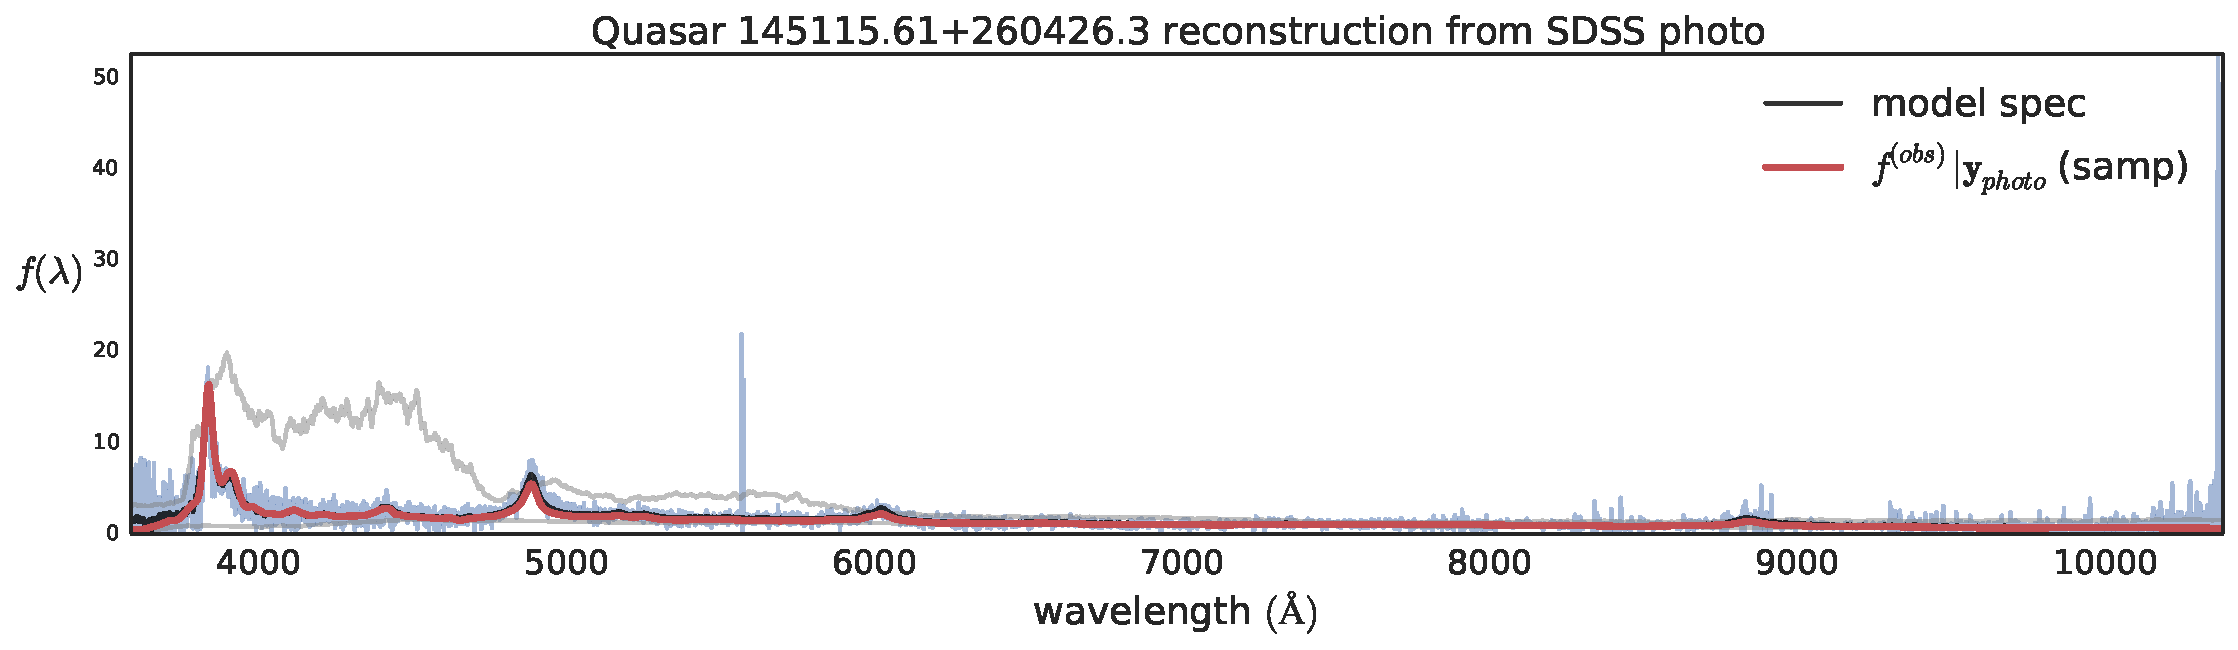
\includegraphics[width=1.5\columnwidth]{../../figs/quasar_plots/close_mid/quasar_282_mcmc_recon}
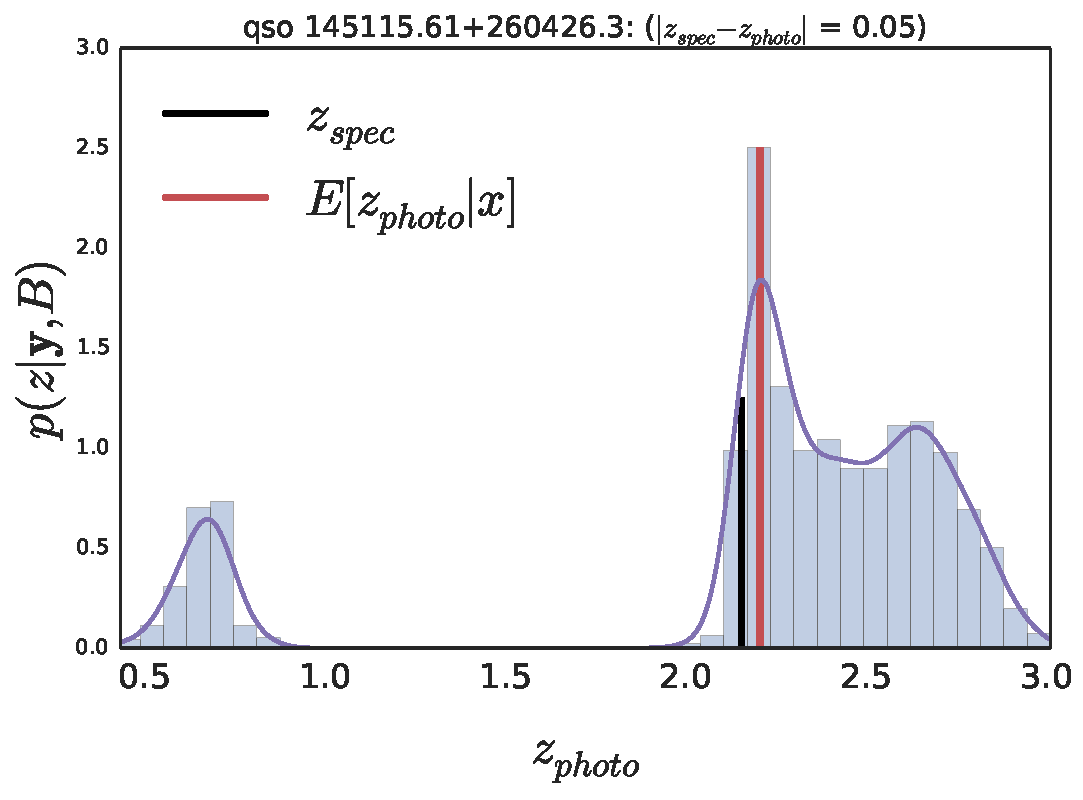
\includegraphics[width=.56\columnwidth]{../../figs/quasar_plots/close_mid/quasar_282_posterior_z}
}
\centerline{
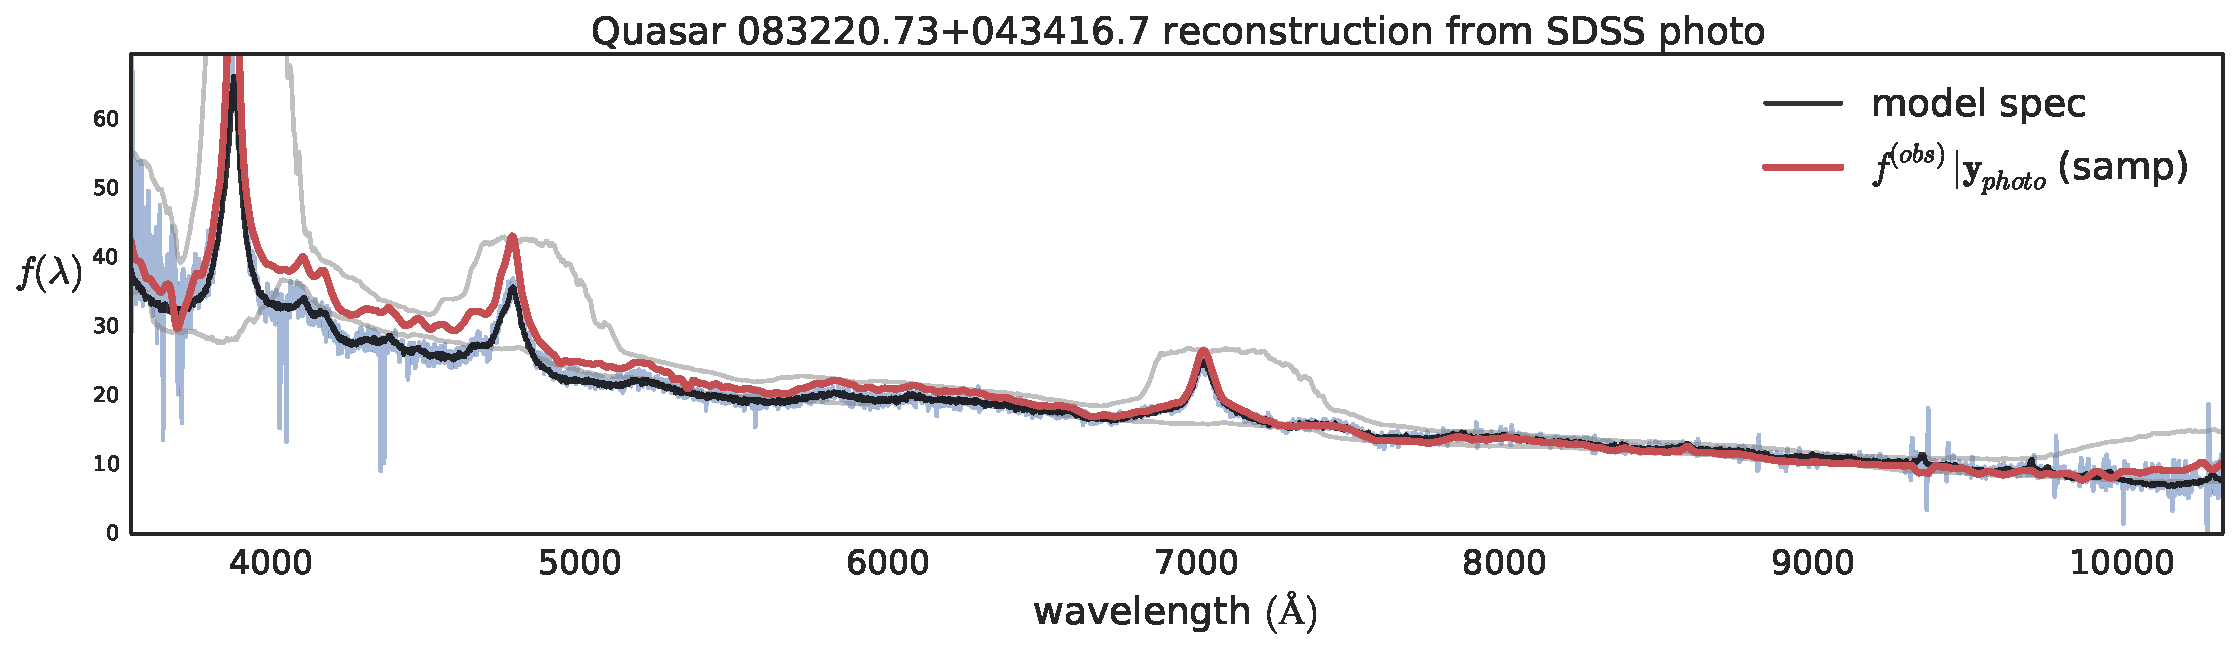
\includegraphics[width=1.5\columnwidth]{../../figs/quasar_plots/close_mid/quasar_1119_mcmc_recon}
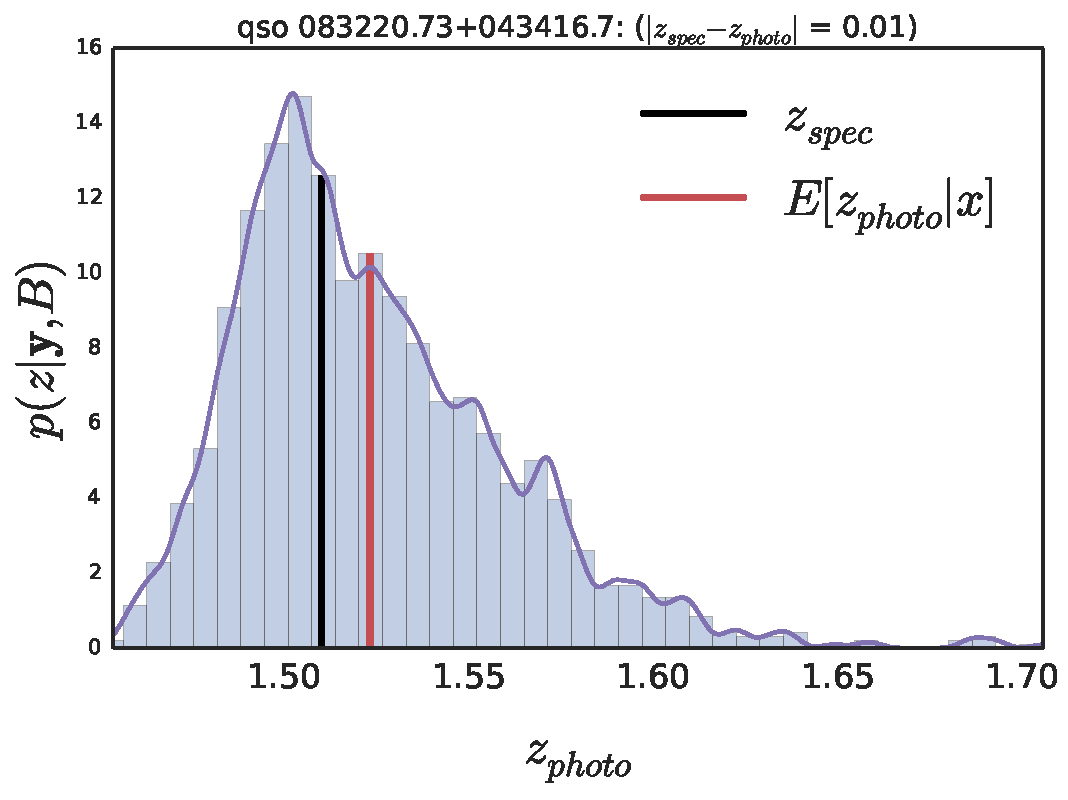
\includegraphics[width=.56\columnwidth]{../../figs/quasar_plots/close_mid/quasar_1119_posterior_z}
}
\centerline{
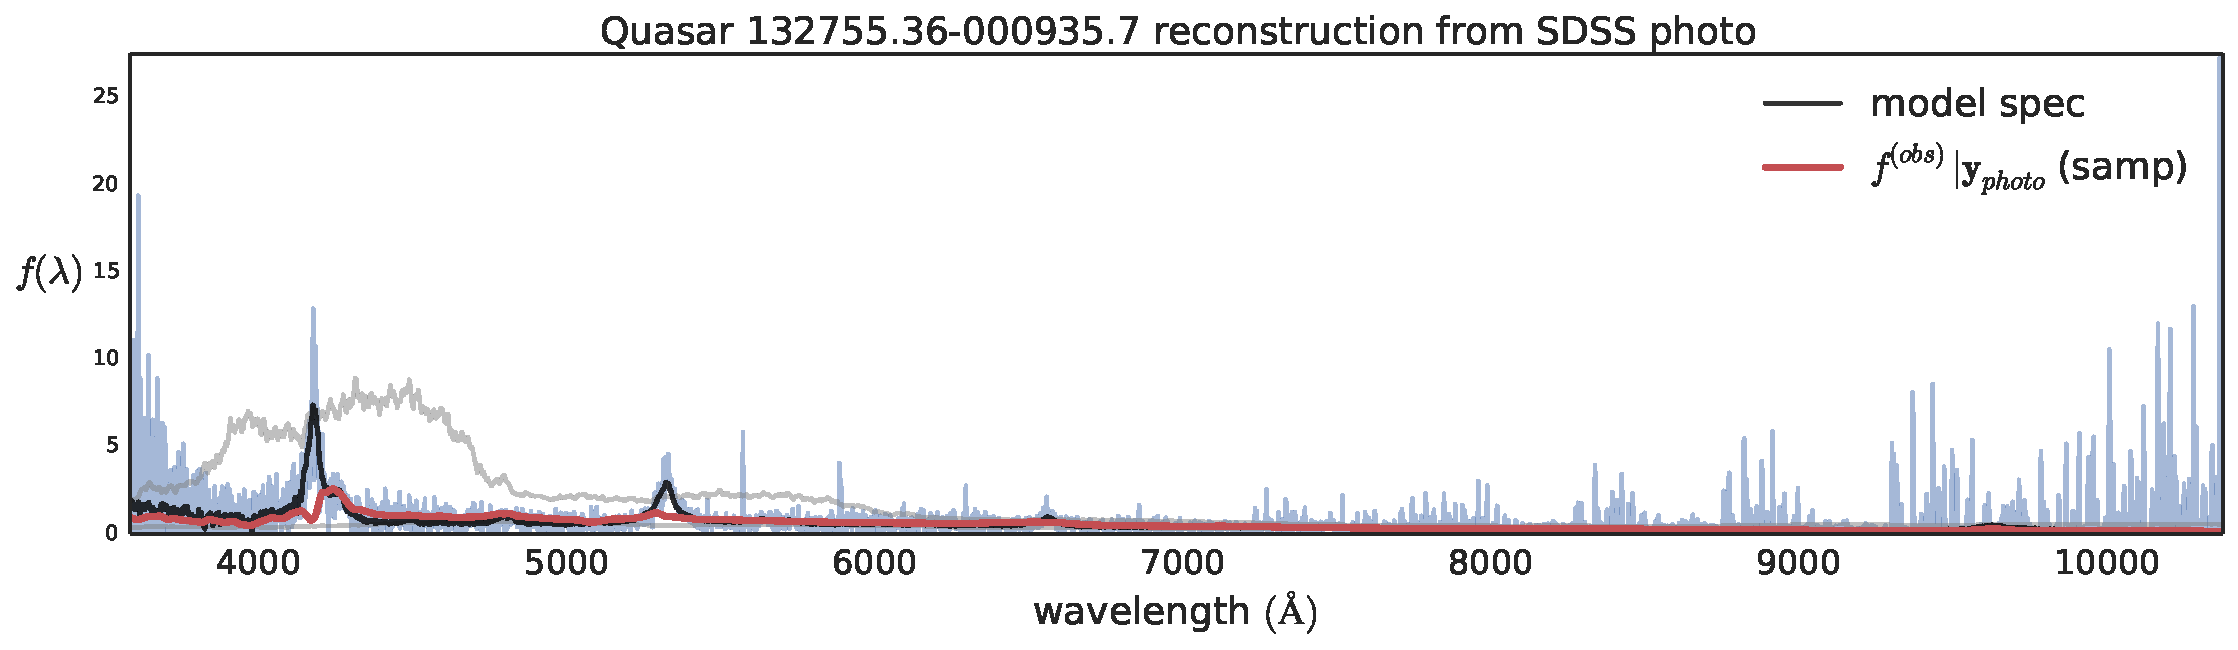
\includegraphics[width=1.5\columnwidth]{../../figs/quasar_plots/close_mid/quasar_1959_mcmc_recon}
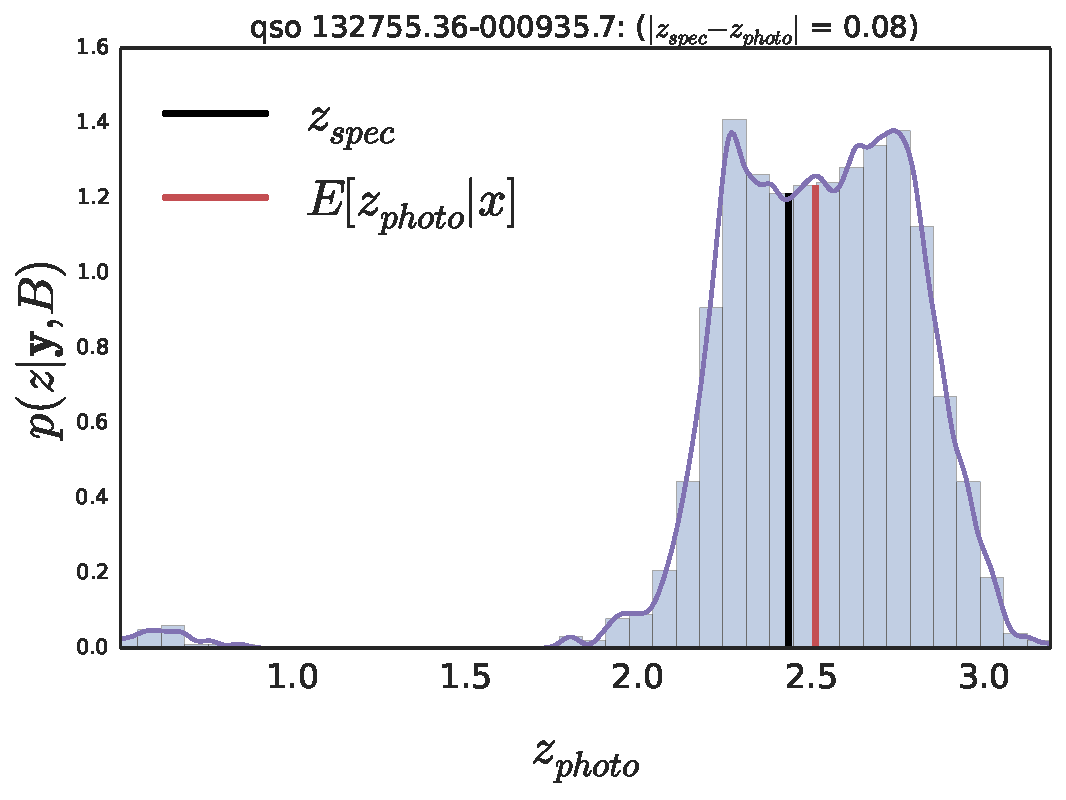
\includegraphics[width=.56\columnwidth]{../../figs/quasar_plots/close_mid/quasar_1959_posterior_z}
}
\vskip -0.2in
\caption{ Three middle range ($1.5 < z < 3$) quasar SEDs.  In red is a sample from the SED posterior that has very close redshift to $z_{spec}$ and corresponding marginal redshift posteriors from photometric data. }
\label{fig:mid}
\vskip -0.2in
\end{figure*}
%---------------
\clearpage

% HI RED SHIFT
%-----  -------------------------------------------------
\begin{figure*}[t]
\centerline{
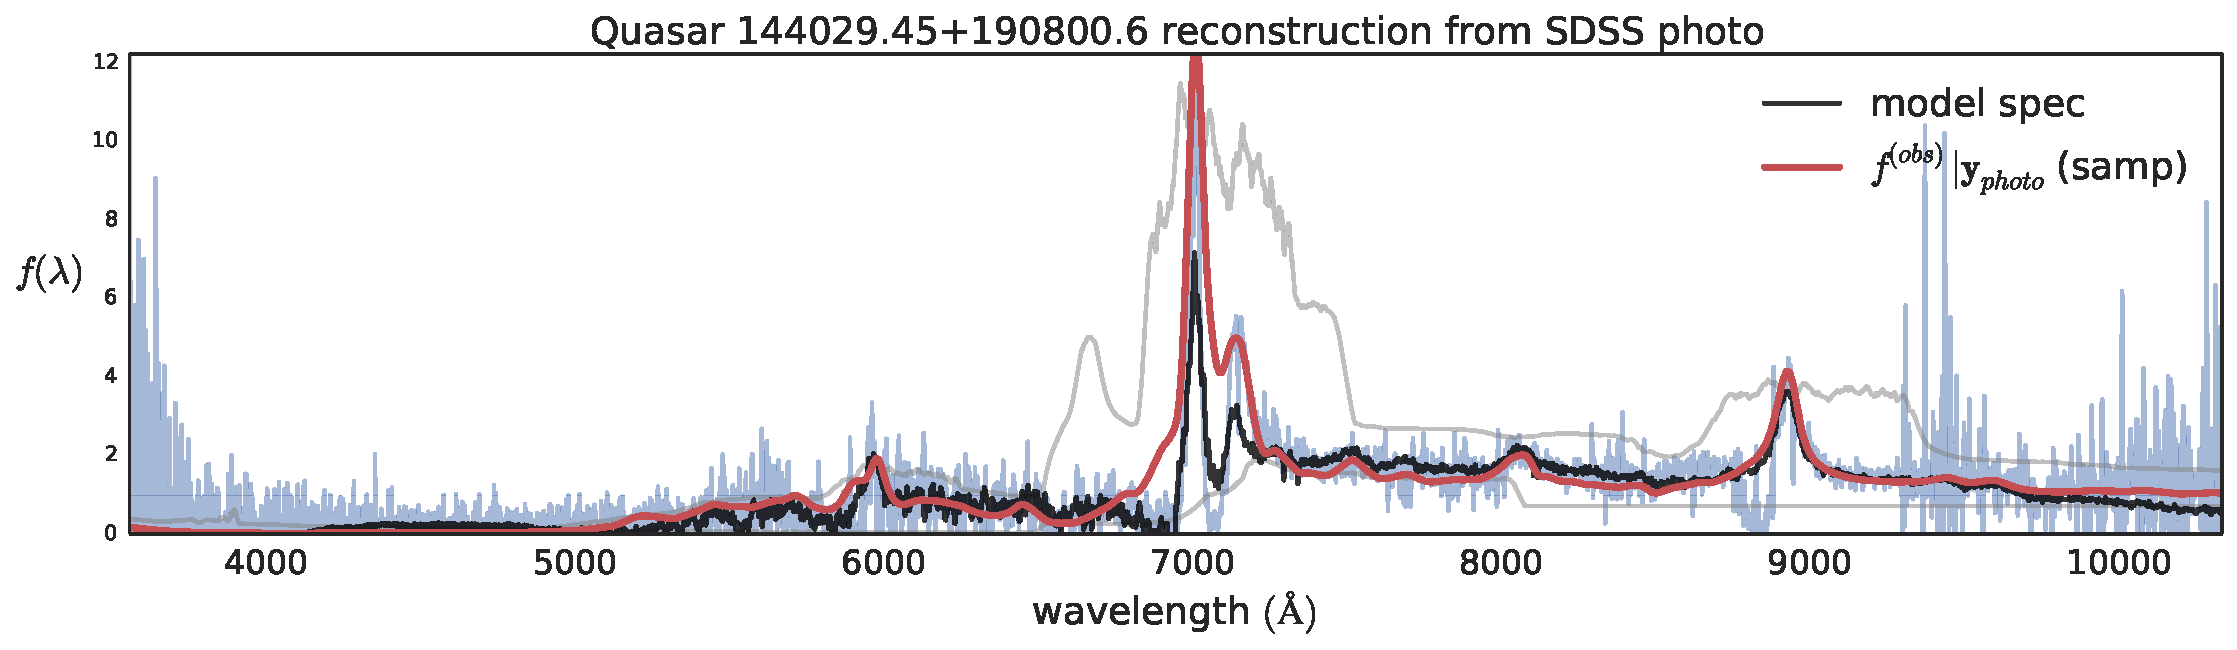
\includegraphics[width=1.5\columnwidth]{../../figs/quasar_plots/close_hi/quasar_248_mcmc_recon}
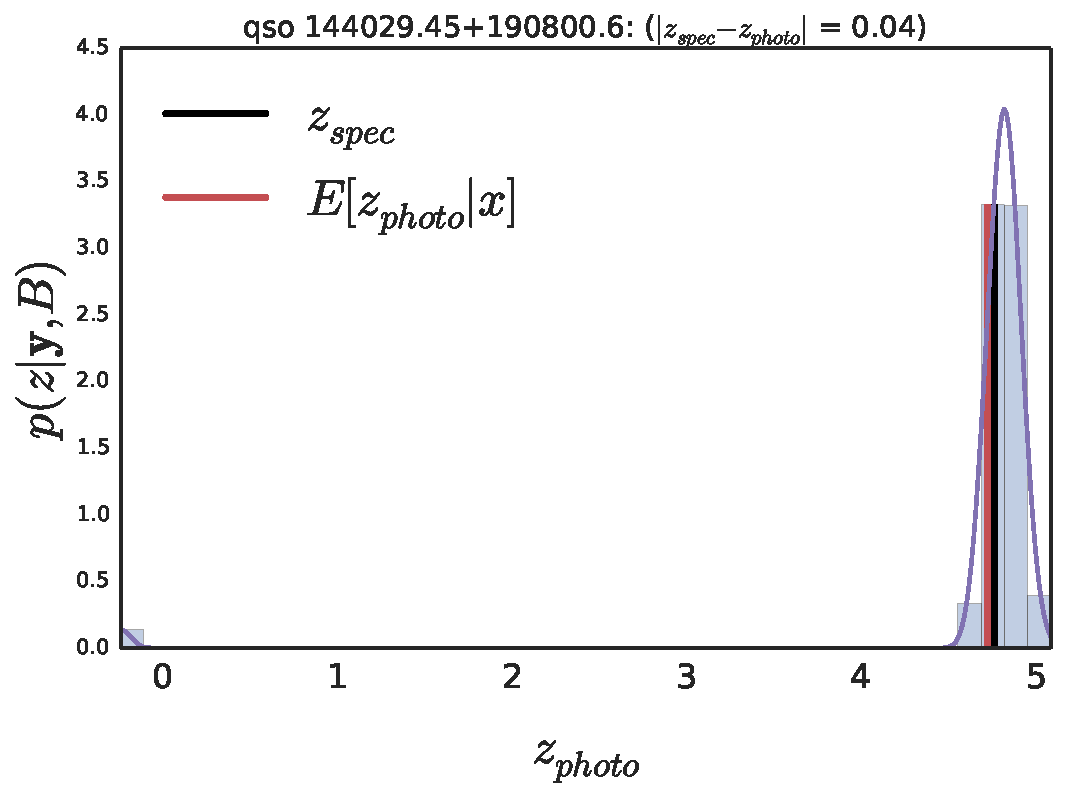
\includegraphics[width=.56\columnwidth]{../../figs/quasar_plots/close_hi/quasar_248_posterior_z}
}
\centerline{
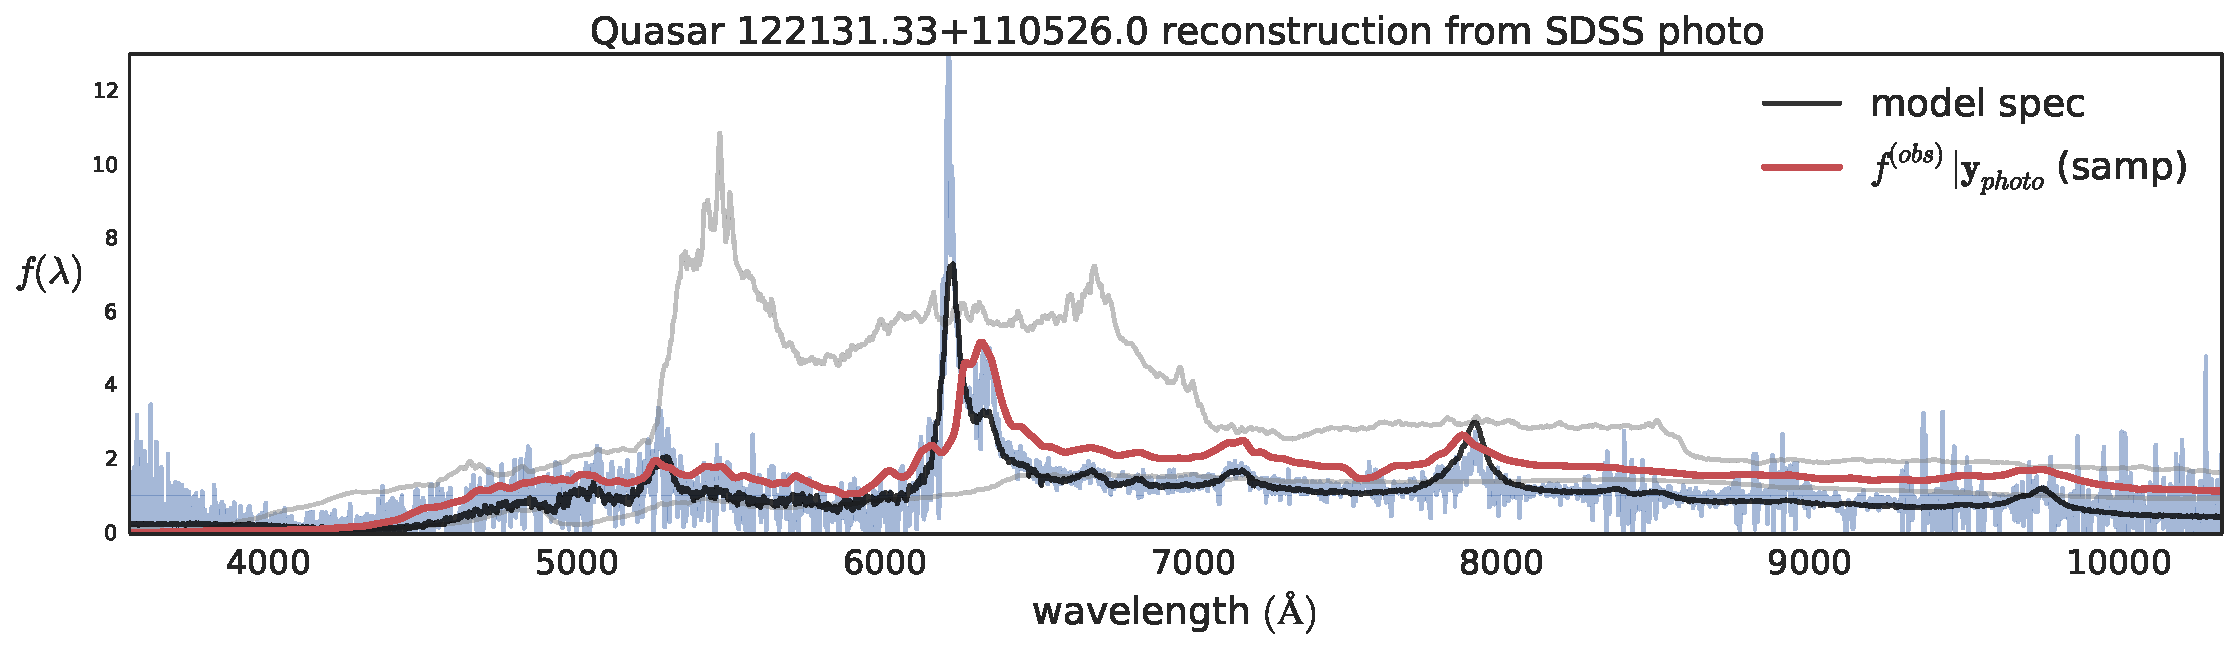
\includegraphics[width=1.5\columnwidth]{../../figs/quasar_plots/close_hi/quasar_1786_mcmc_recon}
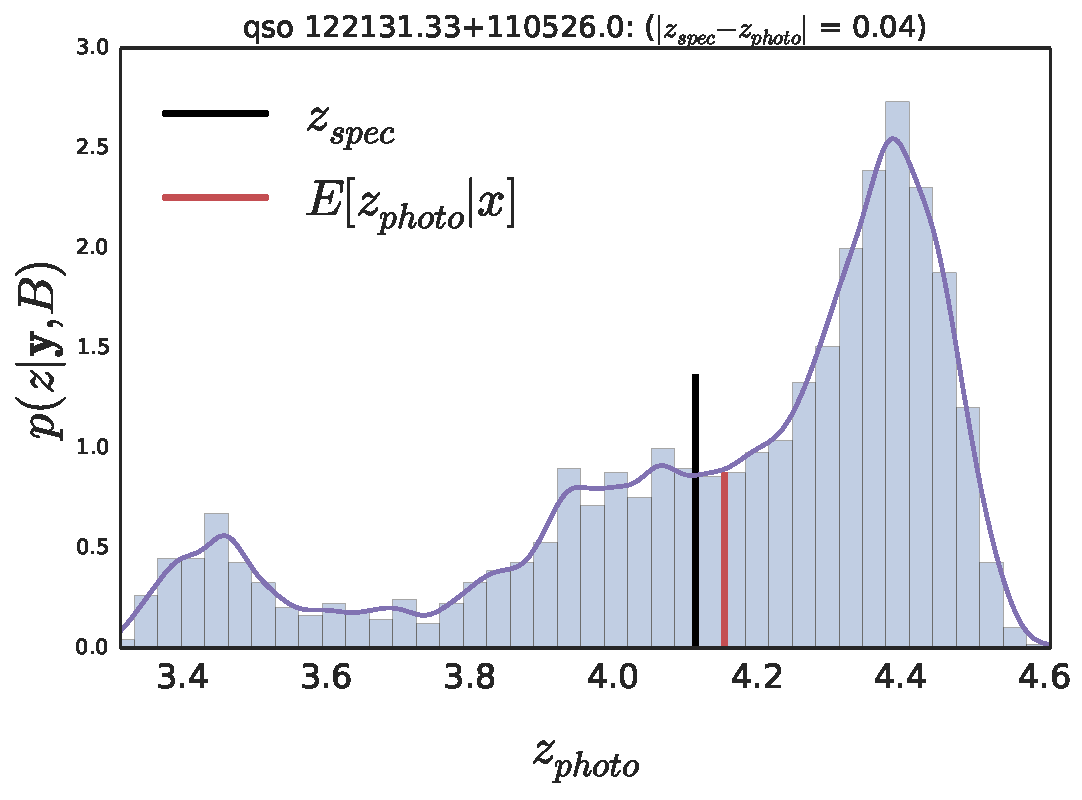
\includegraphics[width=.56\columnwidth]{../../figs/quasar_plots/close_hi/quasar_1786_posterior_z}
}
\centerline{
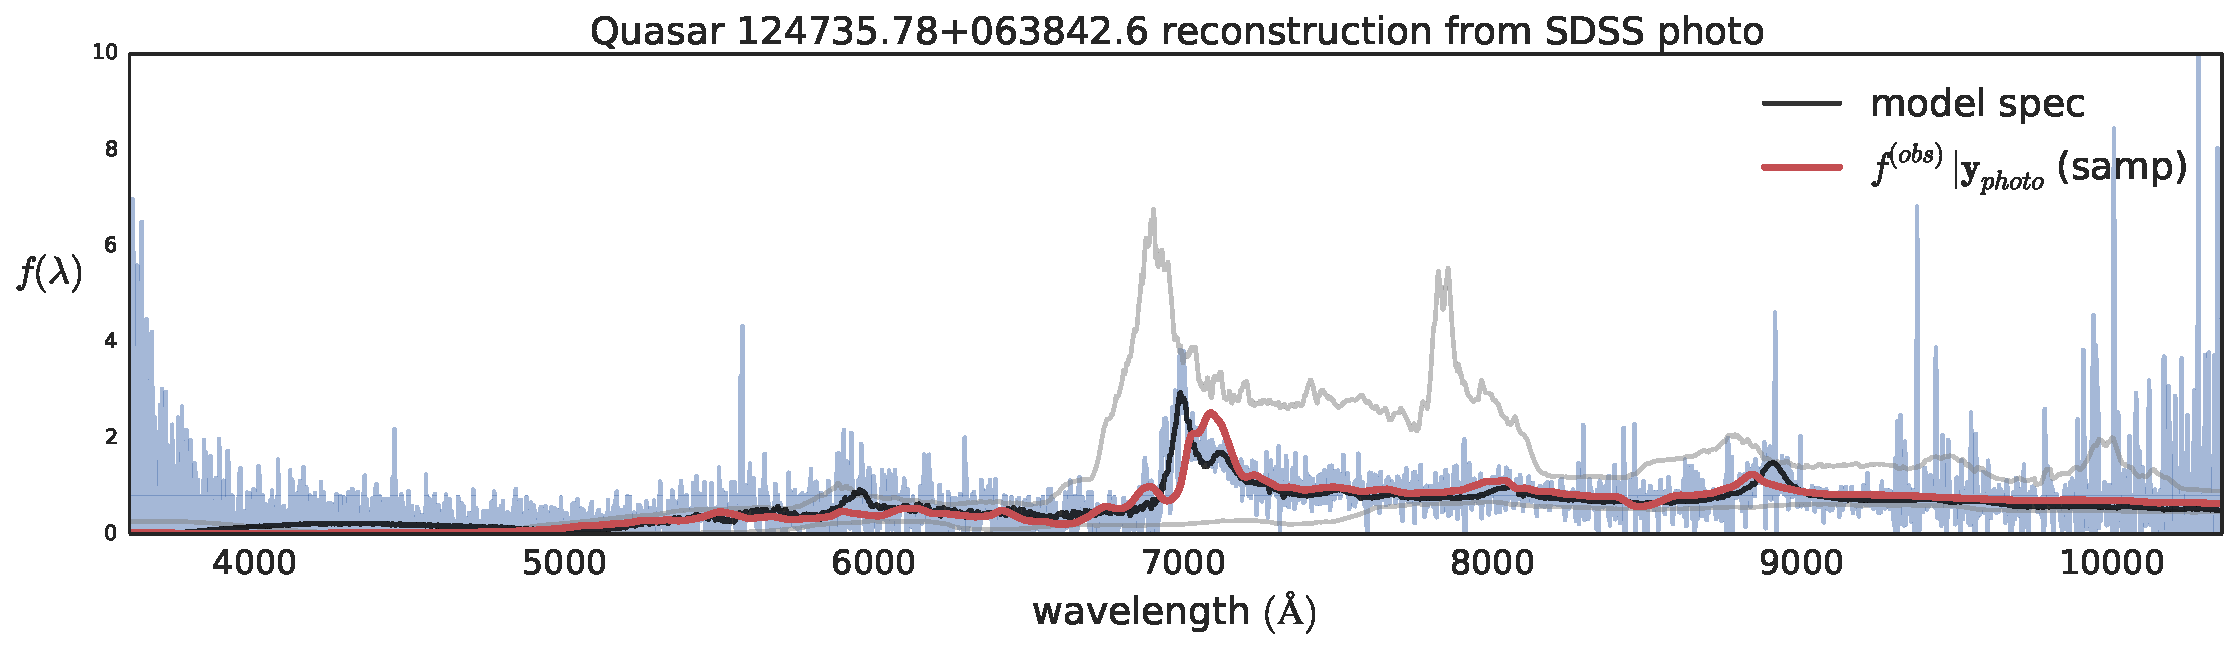
\includegraphics[width=1.5\columnwidth]{../../figs/quasar_plots/close_hi/quasar_1854_mcmc_recon}
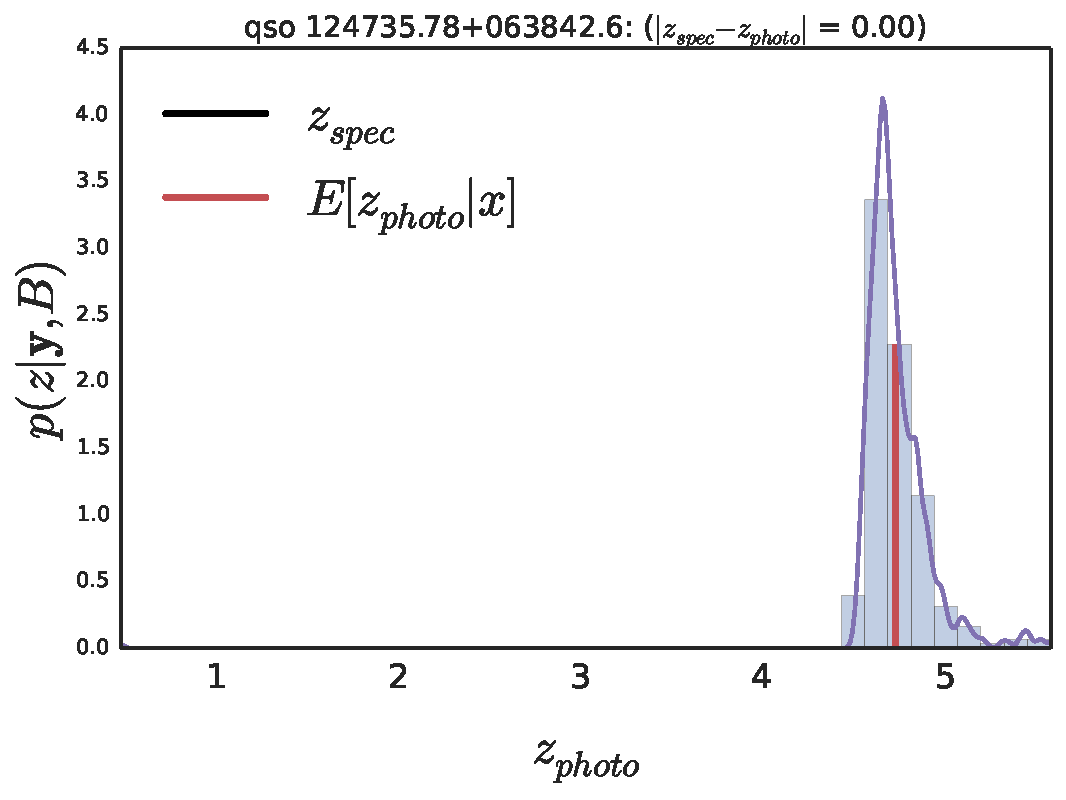
\includegraphics[width=.56\columnwidth]{../../figs/quasar_plots/close_hi/quasar_1854_posterior_z}
}
\vskip -0.2in
\caption{ Three high range ($z > 4$) quasar SEDs.  In red is a sample from the SED posterior that has very close redshift to $z_{spec}$ and corresponding marginal redshift posteriors from photometric data. }
\label{fig:hi}
\vskip -0.2in
\end{figure*}
\clearpage
%---------------



%-----  -------------------------------------------------
\begin{figure*}[t]
\centerline{
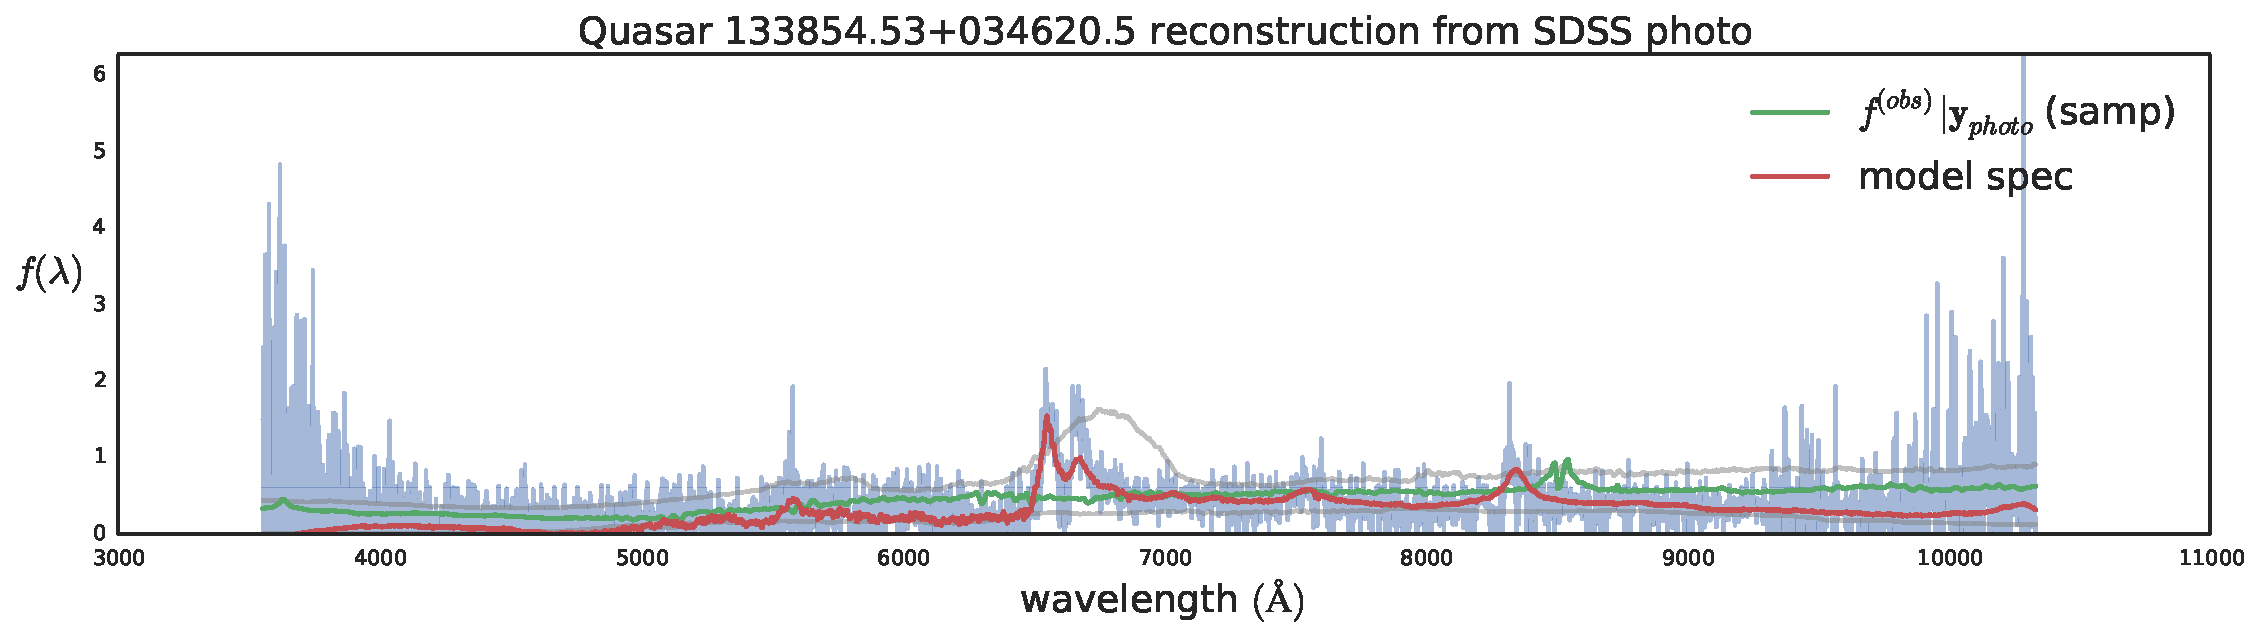
\includegraphics[width=1.5\columnwidth]{../../figs/quasar_plots/quasar_2_mcmc_recon}
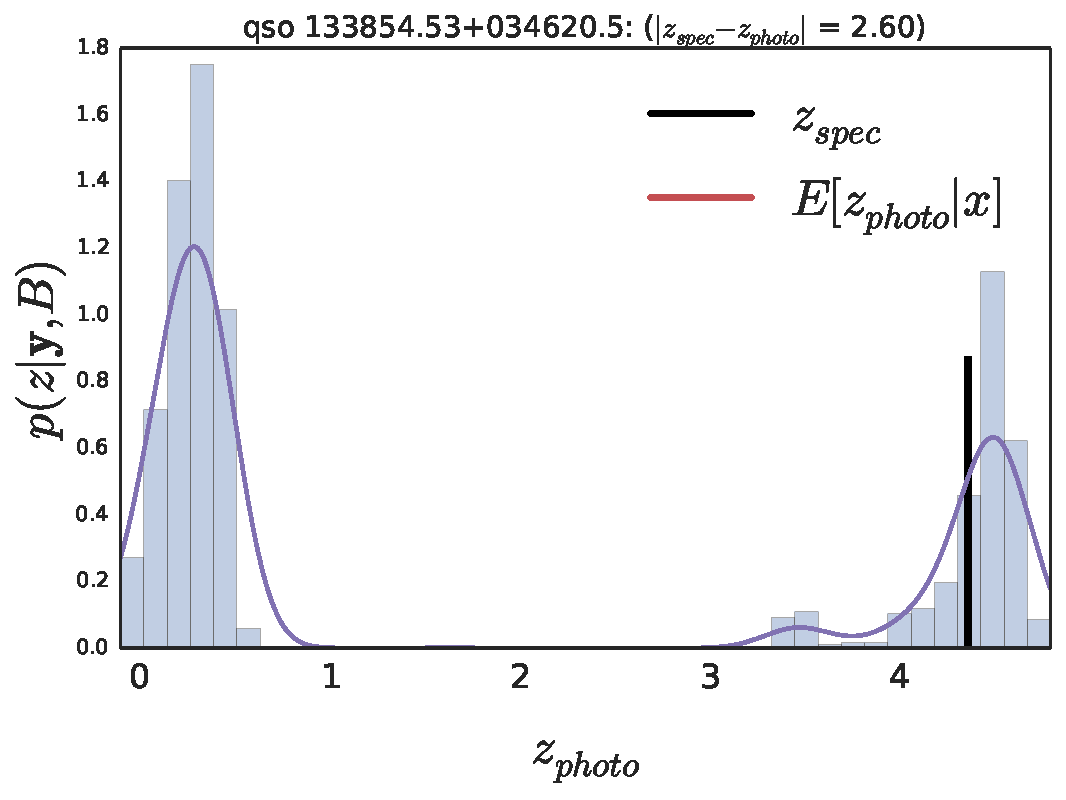
\includegraphics[width=.56\columnwidth]{../../figs/quasar_plots/quasar_2_posterior_z}
}
\centerline{
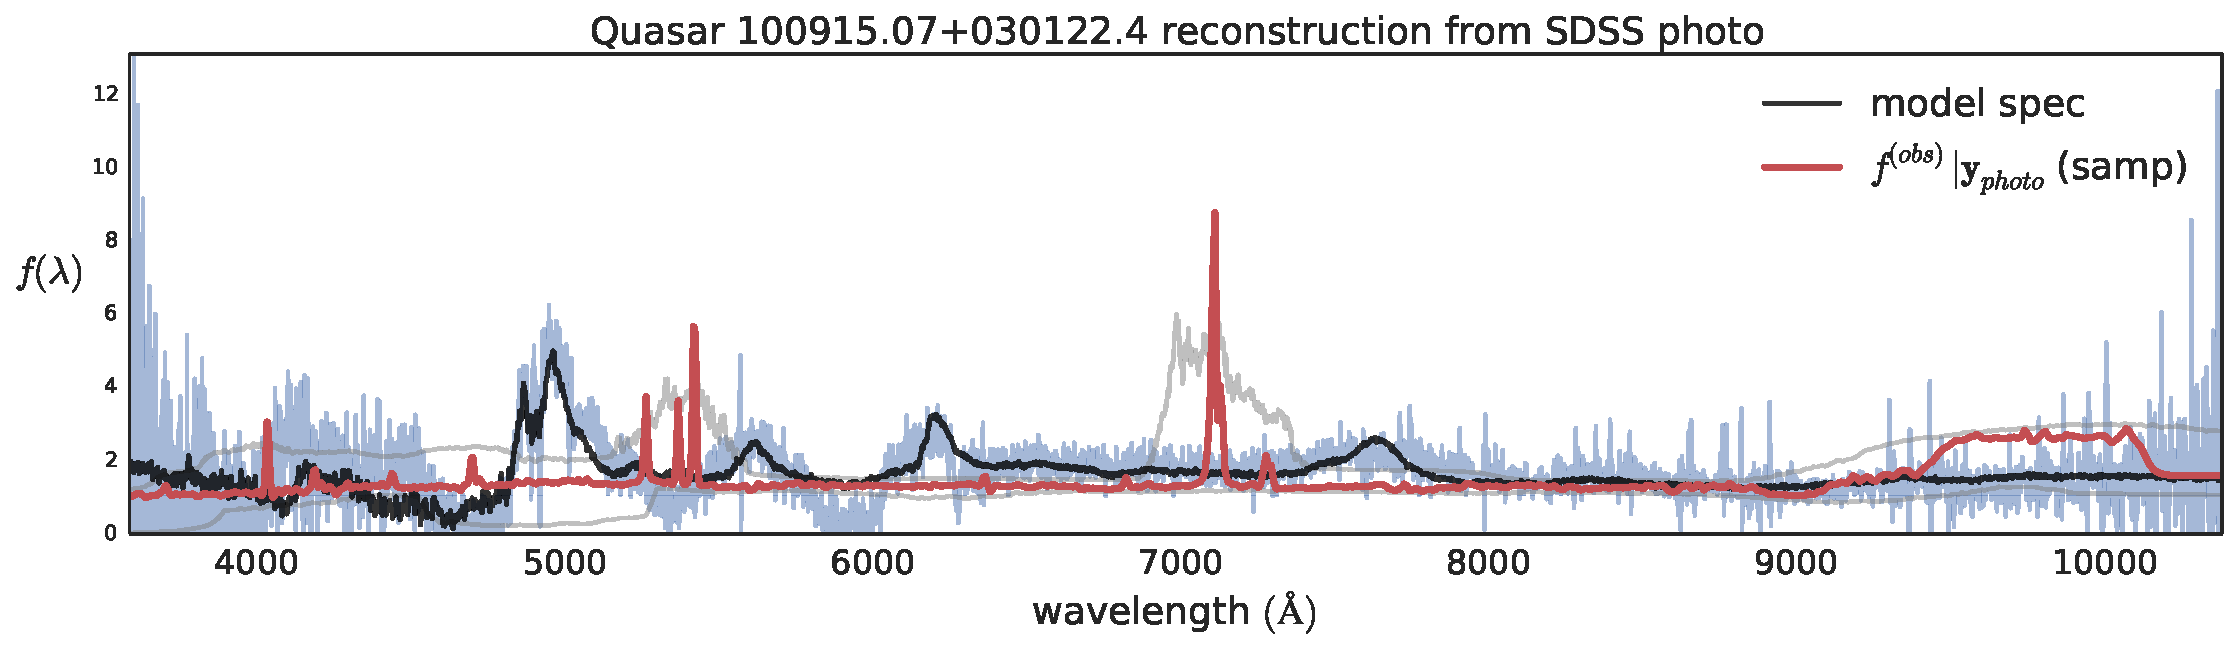
\includegraphics[width=1.5\columnwidth]{../../figs/quasar_plots/quasar_1409_mcmc_recon}
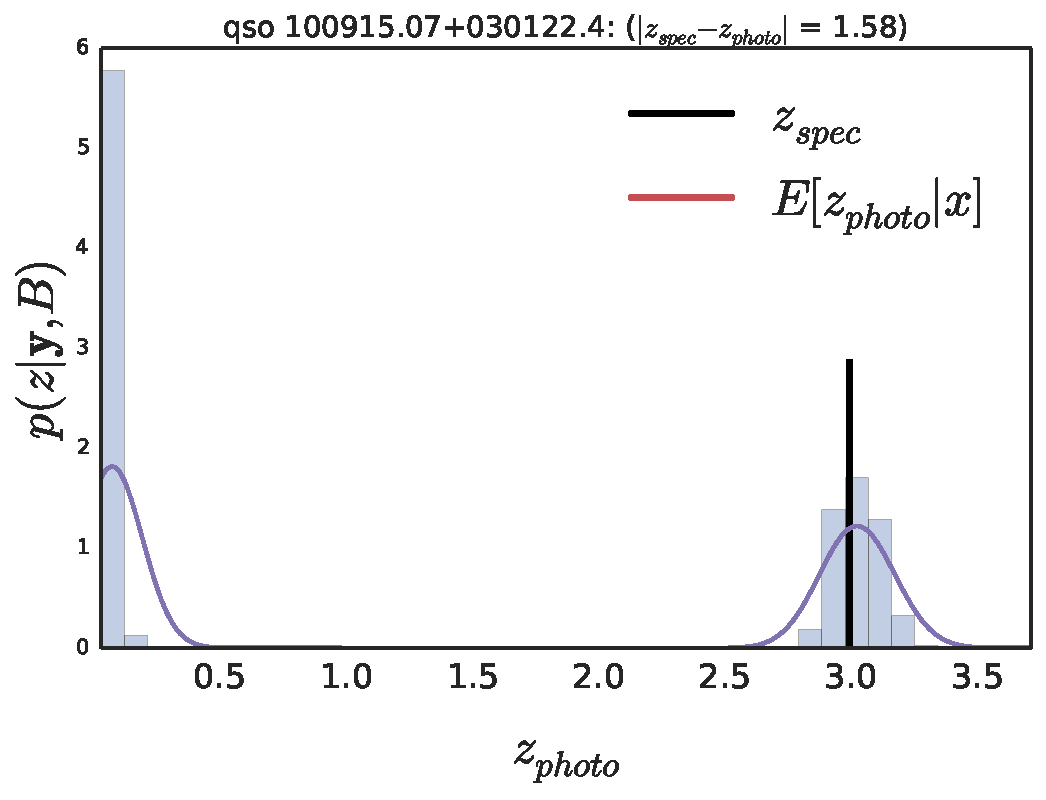
\includegraphics[width=.56\columnwidth]{../../figs/quasar_plots/quasar_1409_posterior_z}
}
\centerline{
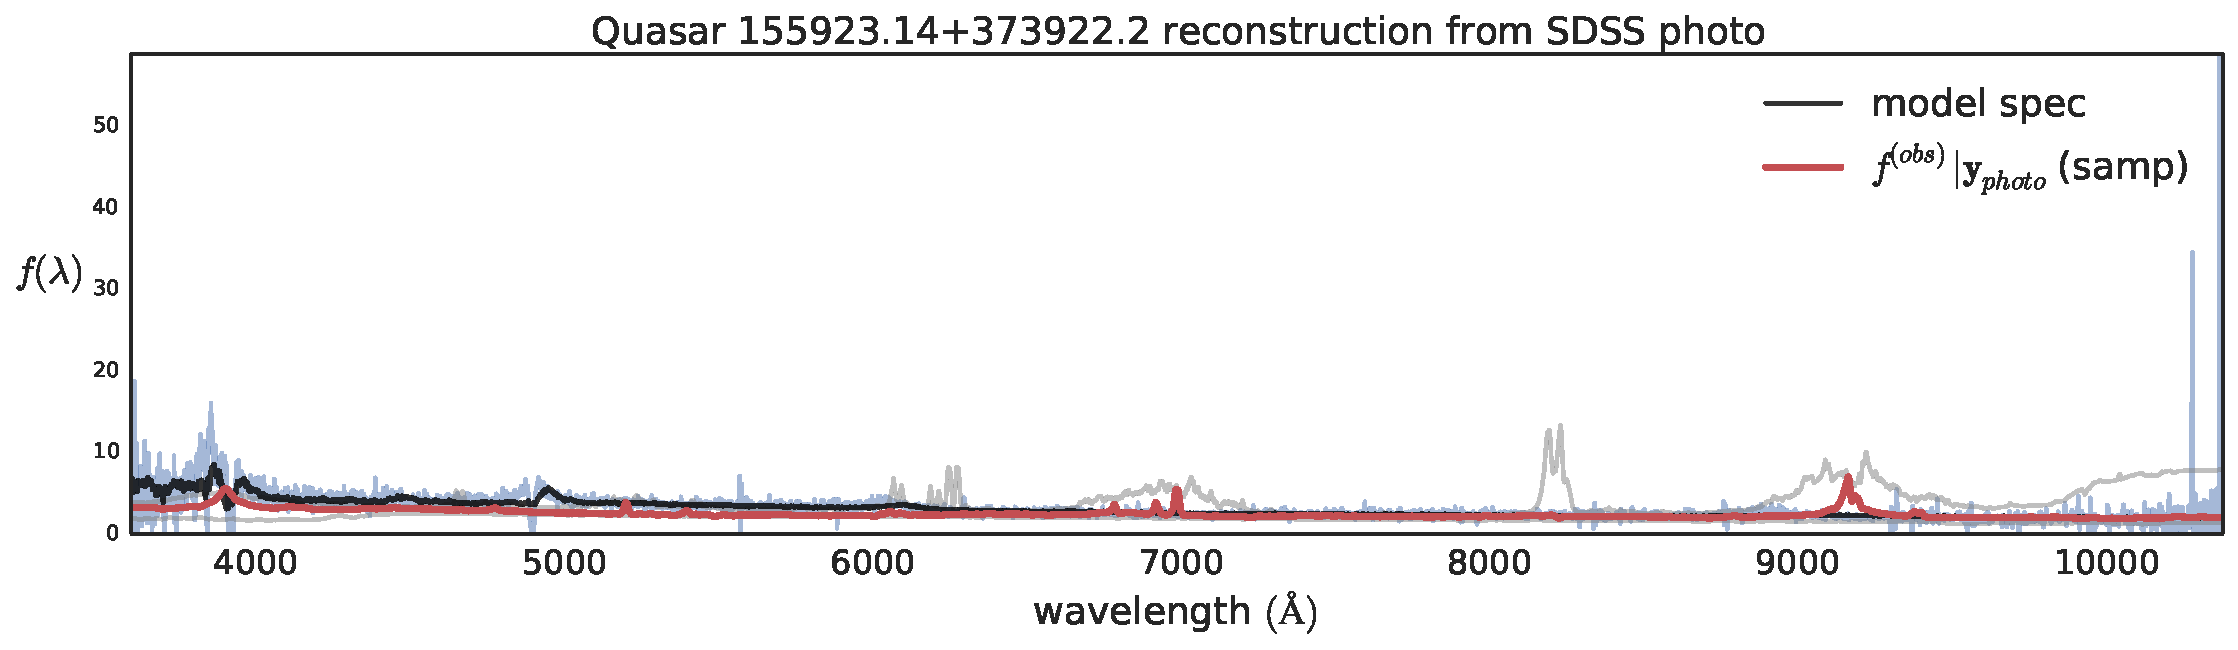
\includegraphics[width=1.5\columnwidth]{../../figs/quasar_plots/quasar_554_mcmc_recon}
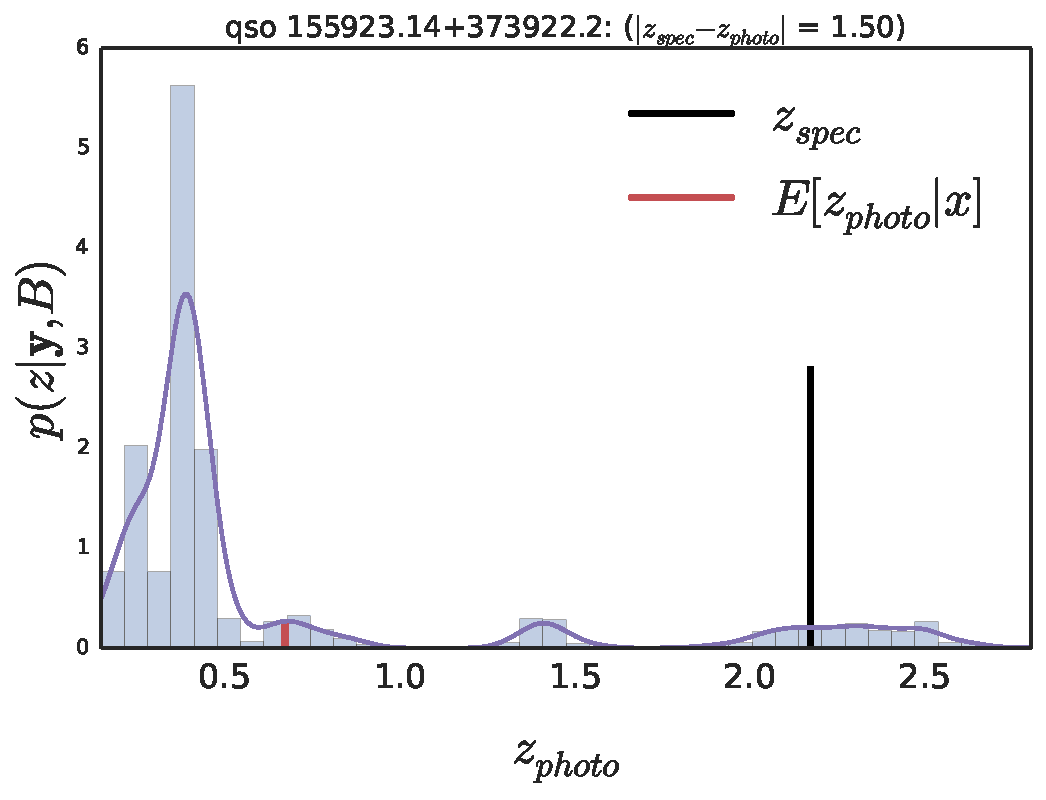
\includegraphics[width=.56\columnwidth]{../../figs/quasar_plots/quasar_554_posterior_z}
}
\vskip -0.2in
\caption{ Three multi-modal distributions and samples from the posterior.}
\label{fig:multi}
\vskip -0.2in
\end{figure*}
%---------------
%
%\bibliography{../refs}
%\bibliographystyle{icml2015}

\end{document} 

